\documentclass[a4paper,10pt]{report}
\usepackage{graphicx}
\usepackage{epstopdf}
\usepackage{ucs}
\usepackage[T1]{fontenc}
\usepackage[utf8x]{inputenc}
\usepackage[english]{babel}

\usepackage{amsmath}
\usepackage[retainorgcmds]{IEEEtrantools}%	IEEEeqnarray

\usepackage{multi row}%	row span in tables

\usepackage{varioref}%	context sensitive references (prints page when far away)
\usepackage{hyperref}%	hyperlinks, references with automatic descriptions
\usepackage{hypcap}

\begin{document}

\tableofcontents

%%%%%%%%%%%%%%%%%%%%%%%%%%%%%%%%%%%%%%%%%%%%%%%
%%% CHAPTER 1: ROOFLINE
%%%%%%%%%%%%%%%%%%%%%%%%%%%%%%%%%%%%%%%%%%%%%%%
\chapter{Roofline}

%%%%%%%%%%%%%%%%%%%%%%%%%%%%%%%%%%%%%%%%%%%%%%%
%%% SECTION 1.1: Profiling
%%%%%%%%%%%%%%%%%%%%%%%%%%%%%%%%%%%%%%%%%%%%%%%
\section{Profiling}
The computer characterized here is the HP dv5-1170ep, released in 2008.

Most of the hardware was obtained from the Intel ARK Website \cite{ark} and from standard Linux tools:
\begin{description}
\item[dmidecode] Tool for hardware dump from BIOS information;
\item[lscpu] Lists CPU information;
\item[lshw] Lists hardware information
\item[getconf] Lists various configuration variables (e.g. cache organization values)
\end{description}

AIDA64 Extreme Edition for Windows 7 was used to measure memory latencies \autoref{fig:aida64}. It's results were then compared against the previosly obtained data to ensure it's accuracy.
Some of the data is theorethically calculated based on the given hardware characteristics. This, of course, represents only a theorethical limit for the hardware, and not actually measured data.

%%%%%%%%%%%%%%%%%%%%%%%%%%%%%%%%%%%%%%%%%%%%%%%
%%% SUBSECTION 1.1.1: Peak FP Performance
%%%%%%%%%%%%%%%%%%%%%%%%%%%%%%%%%%%%%%%%%%%%%%%
\subsection{Peak Floating-Point Performance}
In order to keep coherency with the Roofline paper (see \cite{roofline}), Peak FP Performance was measured using double-precision floating point numbers. The formula to calculate the maximum double precision floating point throughput is:

$$\mathrm{Flop/s_{max}} = T_{\mathrm{FP}} \times f_{\mathrm{clock}} \times \#_{\mathrm{cores}}$$

Where $T_{\mathrm{FP}}$ is the double precision floating point throughput of each core.

The CPU in question, Core 2 Duo P8600, has two cores working with a clock rate of 2.4 GHz. Being based on the Core micro architecture, each core has one execution unit for 128-bit floating point addition, and one for multiplication. When considering SIMD operations, with the SSE and MMX extensions, then each 128-bit register can carry two double precision floating point values, thus effectively doubling the throughput. With an ideal multiply/add balance, four floating point operations can run in parallel.

\begin{IEEEeqnarray}{CrClC}
\Rightarrow		& \mathrm{Flop/s_{max}} & = & 4 \times \left (2.4 \times 10^9 \right ) \times 2 & \Leftrightarrow	\nonumber \\
\Leftrightarrow	& \mathrm{Flop/s_{max}} & = & 19.2\;\mathrm{GFlop/s} & \nonumber
\end{IEEEeqnarray}

%%%%%%%%%%%%%%%%%%%%%%%%%%%%%%%%%%%%%%%%%%%%%%%
%%% SUBSECTION 1.1.2: Peak Mem BW
%%%%%%%%%%%%%%%%%%%%%%%%%%%%%%%%%%%%%%%%%%%%%%%
\subsection{Peak Memory Bandwidth}
This value can be calculated based on the memory clock rate and the memory bus. Multiple channels should also be taken into account.
The memory is a SDRAM DDR2 operating at a clock rate of 800MHz, and using two modules, taking advantage of the dual-channel. The bus width is 64 bits (or 8 Bytes)

\begin{IEEEeqnarray}{CrClC}
\Rightarrow		& \mathrm{BW_{max}} & = & MEM_{\mathrm{clock}} \times bus_{\mathrm{width}} \times \#\mathrm{channels} & \Leftrightarrow \\
\Leftrightarrow	& \mathrm{BW_{max}} & = & (800 \times 10^9) \times 64 \times 2 & \Leftrightarrow \nonumber \\
\Leftrightarrow & \mathrm{BW_{max}} & = & 12.8\;\mathrm{GB/s} & \nonumber
\end{IEEEeqnarray}


%%%%%%%%%%%%%%%%%%%%%%%%%%%%%%%%%%%%%%%%%%%%%%%
%%% SUBSECTION 1.2.3: Summary
%%%%%%%%%%%%%%%%%%%%%%%%%%%%%%%%%%%%%%%%%%%%%%%
\subsection{Summary}
The full characterization of the laptop is summarized in \autoref{tab:profile}

\begin{table}[!htp]
	\begin{center}
		\begin{tabular}{|lrl|}
			\hline
			\multicolumn{2}{|l}{\textbf{Manufacturer:}}	&	HP					\\
			\multicolumn{2}{|l}{\textbf{Model:}}		&	Pavilion dv5 1170ep	\\
			\hline
			\hline

			\textbf{Processor:}	&						&						\\
			%\cline{2-3}
			\multicolumn{1}{|c}{\multirow{6}{*}}
				&	Manufacturer:			&	Intel							\\
				&	Model:					&	P8600							\\
				&	$\mu$-arch				&	Core							\\
				&	Clock frequency			&	2.4 GHz							\\
				&	Cores					&	2								\\
				&	Threads:				&	2								\\
				&	Peak Flop/s				&	19.2 GFlop/s					\\
			\hline
			\hline

			\textbf{Cache:}	&						&						\\
			\multicolumn{1}{|c}{\multirow{2}{*}{L1}}
				&	Scope			&	Core		\\
				&	Size			&	32KB + 32KB	\\
				&	Associativity	&	8-way		\\
				&	Line Size		&	64 B		\\
				&	Write Policy	&	Write-back	\\
			\hline
			\multicolumn{1}{|c}{\multirow{2}{*}{L2}}
				&	Scope			&	shared		\\
				&	Size			&	3MB			\\
				&	Associativity	&	12-way		\\
				&	Line Size		&	64 B		\\
				&	Write Policy	&	Write-back	\\
			\hline
			\hline

			\textbf{Main Memory:}	&				&					\\
			\multicolumn{1}{|c}{\multirow{6}{*}}
				&	Type			&	SDRAM DDR2 PC6400				\\
				&	Frequency		&	800 MHz							\\
				&	Num. Channels	&	2								\\
				&	Size			&	4 GB							\\
				&	Latency			&	81.1 ns \autoref{fig:aida64}	\\
				&	Peak Bandwith	&	12.8 GB/s						\\
			\hline			
		\end{tabular}
	\end{center}
	\label{tab:profile}
\end{table}


\begin{figure}[!htp]
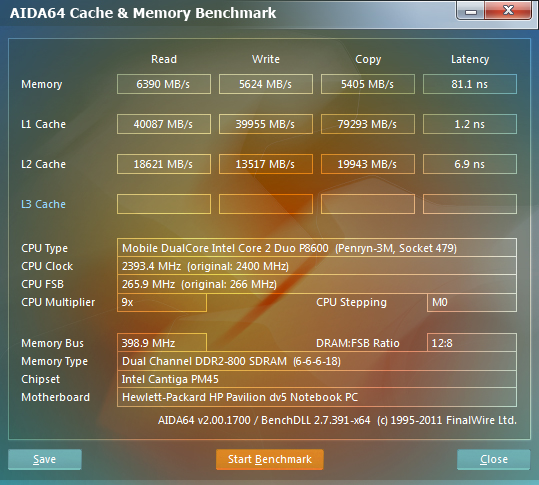
\includegraphics[width=12cm]{images/aida64.png}
\label{fig:aida64}
\caption[Memory benchmark]{Memory benchmark with Aida64 Extreme Edition}
\end{figure}

\chapter{Roofline}

\section{Profile}

\subsection{Laptop}

\subsubsection{Summary}

The collected and calculated information is summarized in \autoref{tab:profile}.

\begin{table}[!htp]
	\begin{center}
		\begin{tabular}{l r l}
		\hline\hline
		\multicolumn{2}{l}{\textbf{Manufacturer:}} & Apple	\\
		\multicolumn{2}{l}{\textbf{Model:}} & MacBook Pro 6,2	\\
		\hline
		\textbf{Processors:} & &	\\
		\cline{2-3}
		\multicolumn{1}{c}{\multirow{7}{*}{1x}}
		& Manufacturer: & Intel	\\
		& Model: & i5-540M	\\
		& Clock frequency: & 2.4 GHz	\\
		& Cores: & 2	\\
		& Threads: & 4	\\
		& Max. mem. bandwidth: & 17.1 GB/s	\\
		& Peak Flop/s: & 19.2 GFlop/s	\\
		\hline
		\textbf{Cache:} & &	\\
		\cline{2-3}
		& Scope: & core	\\%	L1 scope
		& Size: & 32 KB + 32 KB	\\%	L1 cache size
		\cline{2-3}
		& Scope: & core	\\%	L2 scope
		& Size: & 256 KB	\\%	L2 cache size
		\cline{2-3}
		& Scope: & shared	\\%	L3 scope
		& Size: & 3 MB	\\%	L3 cache size
		\hline
		\textbf{Memory:} & &	\\
		& Type: & DDR3	\\
		& Frequency: & 1067 MHz	\\
		& Size: & 4 GB	\\
		& Latency: & ≈ 101.1 ns	\\
		& Peak bandwidth: & 17.07 GB/s	\\
		\hline\hline
		\end{tabular}
	\end{center}
	\caption[Macbook Pro 15"]{Laptop hardware profile (official datasheet, benchmark results and optimum calculated values)}
	\label{tab:profile}
\end{table}

Apple MacBook Pro 6,2

CPU
1 Intel Core i5-520M
2 cores/processador
2 threads/core

Memória:
4 GB
latência: 16 ciclos

Peak FLOPS:

2 unidades de execução por core, 2 cores, superescalares com capacidade de submeter duas instruções SIMD por ciclo, aproveitando as unidades de execução em pleno => 4 FLOP / ciclo

\subsubsection{System Information}
The 


Using the utility \textit{System Information}, installed by default with \textit{Mac OS X Lion}, we can obtain the model  (\texttt{MacBook Pro}

\begin{description}
\item[Manufacturer:]{Apple}
\item[Model:]{MacBook Pro 6,2}
\item[CPU:]{Intel i5-540M 2.4 GHz
	\begin{itemize}
	\item[1x]{processor}
	\item[2x]{cores}
	\item[4$\times$]{threads}
	\end{itemize}
}
\item[Memory:]{4GB DDR3 1067MHz
	\begin{description}
	\item[Latency]{
	Using AIDA64 benchmarking software (see \autoref{fig:aida64}) it's possible to know the \textit{Column Access Strobe} time:
		$$\mathrm{tCAS} = 7$$
	measured in memory clock cycles.
	
	That value can be converted to nanoseconds:
		$$\mathrm{tCAS}_{\Delta t} = \left( \frac{\mathrm{tCAS}}{f_{\mathrm{MHz}}} \right) \times 1000$$
	
	Using the processor clock frequency, we can calculate the clock cycle time:

	%\begin{IEEEeqnarray}{CrClC}
		%& f & = & 2.4\;\mathrm{GHz} & \Leftrightarrow	\nonumber\\
		%\Leftrightarrow & T & = & 4.17 \times 10^{-9}\;\mathrm{s}	\nonumber\\
		%& & = & 4.17 \times 10^{-1}\;\mathrm{ns}$$	\nonumber
	%\end{IEEEeqnarray}
	}
	\end{description}
}
\end{description}

\begin{figure}[!htp]
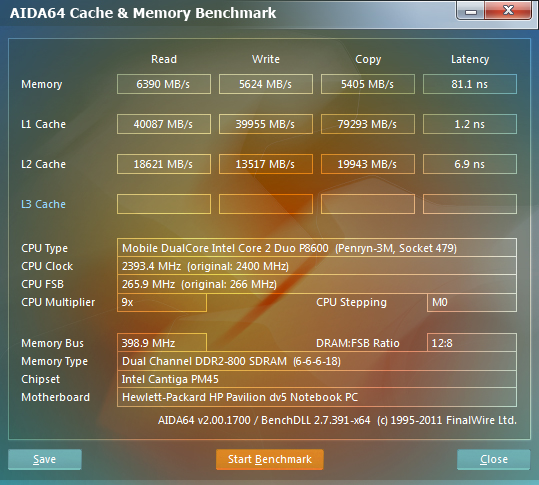
\includegraphics[width=12cm]{images/aida64.png}
\label{fig:aida64}
\caption[Memory benchmark]{Memory benchmark with Aida64 Extreme Edition}
\end{figure}

\appendix

%%%%%%%%%%%%%%%%%%%%%%%%%%%%%%%%%%%%%%%%%%%%%%%
%%% BIBLIOGRAPHY
%%%%%%%%%%%%%%%%%%%%%%%%%%%%%%%%%%%%%%%%%%%%%%%
\begin{thebibliography}{9}
\bibitem{roofline}
	\texttt{\small
	Roofline: An insightful Visual Performance Model for Floating-Point Programs and Multicore Architectures}	\\
	\emph{Samuel Webb Williams, Andre Waterman, David A. Patterson}	\\
	28th November 2011

\bibitem{ark}
	\texttt{\small
	http://ark.intel.com/products/35568/Intel-Core2-Duo-Processor-P8600}	\\
	\emph{Intel{\textregistered} Core 2 Duo{\texttrademark} P8600}	\\
	{\copyright}Intel Corporation	\\
	28th November 2011

\bibitem{intelmanual}
	\texttt{\small
	Intel{\textregistered} 64 and IA-32 Architectures Software Developer Manuals}	\\
	{\copyright}Intel Corporation	\\
	29th November 2011

\end{thebibliography}

\end{document}
